\documentclass[10pt]{exam}
\usepackage[icp]{template-for-exam}
\usepackage{tikz}
\usepackage[top=0.2in, bottom=0.5in, left=1in, right=1in]{geometry}


\begin{document}
\pagestyle{empty}

\def\mytitle{C2 (Gas Laws) Test}

\newcommand{\topmatter} {
  {\Large \mytitle}
}
\newcommand{\bottommatter}{

  \paragraph{Question 26}
  Pick one of the gas laws (Boyle's pressure--volume law, Charles' volume--temperature law, or Gay-Lussac's pressure--temperature law) and explain why it makes sense.  Make sure to explain what is happening to the particles in the gas.

  \fillwithdottedlines{15em}


}

\newcommand{\drawscantron}[2]{
  \begin{flushright}
    \begin{tikzpicture}
      \node[anchor=south west] at (0,0) {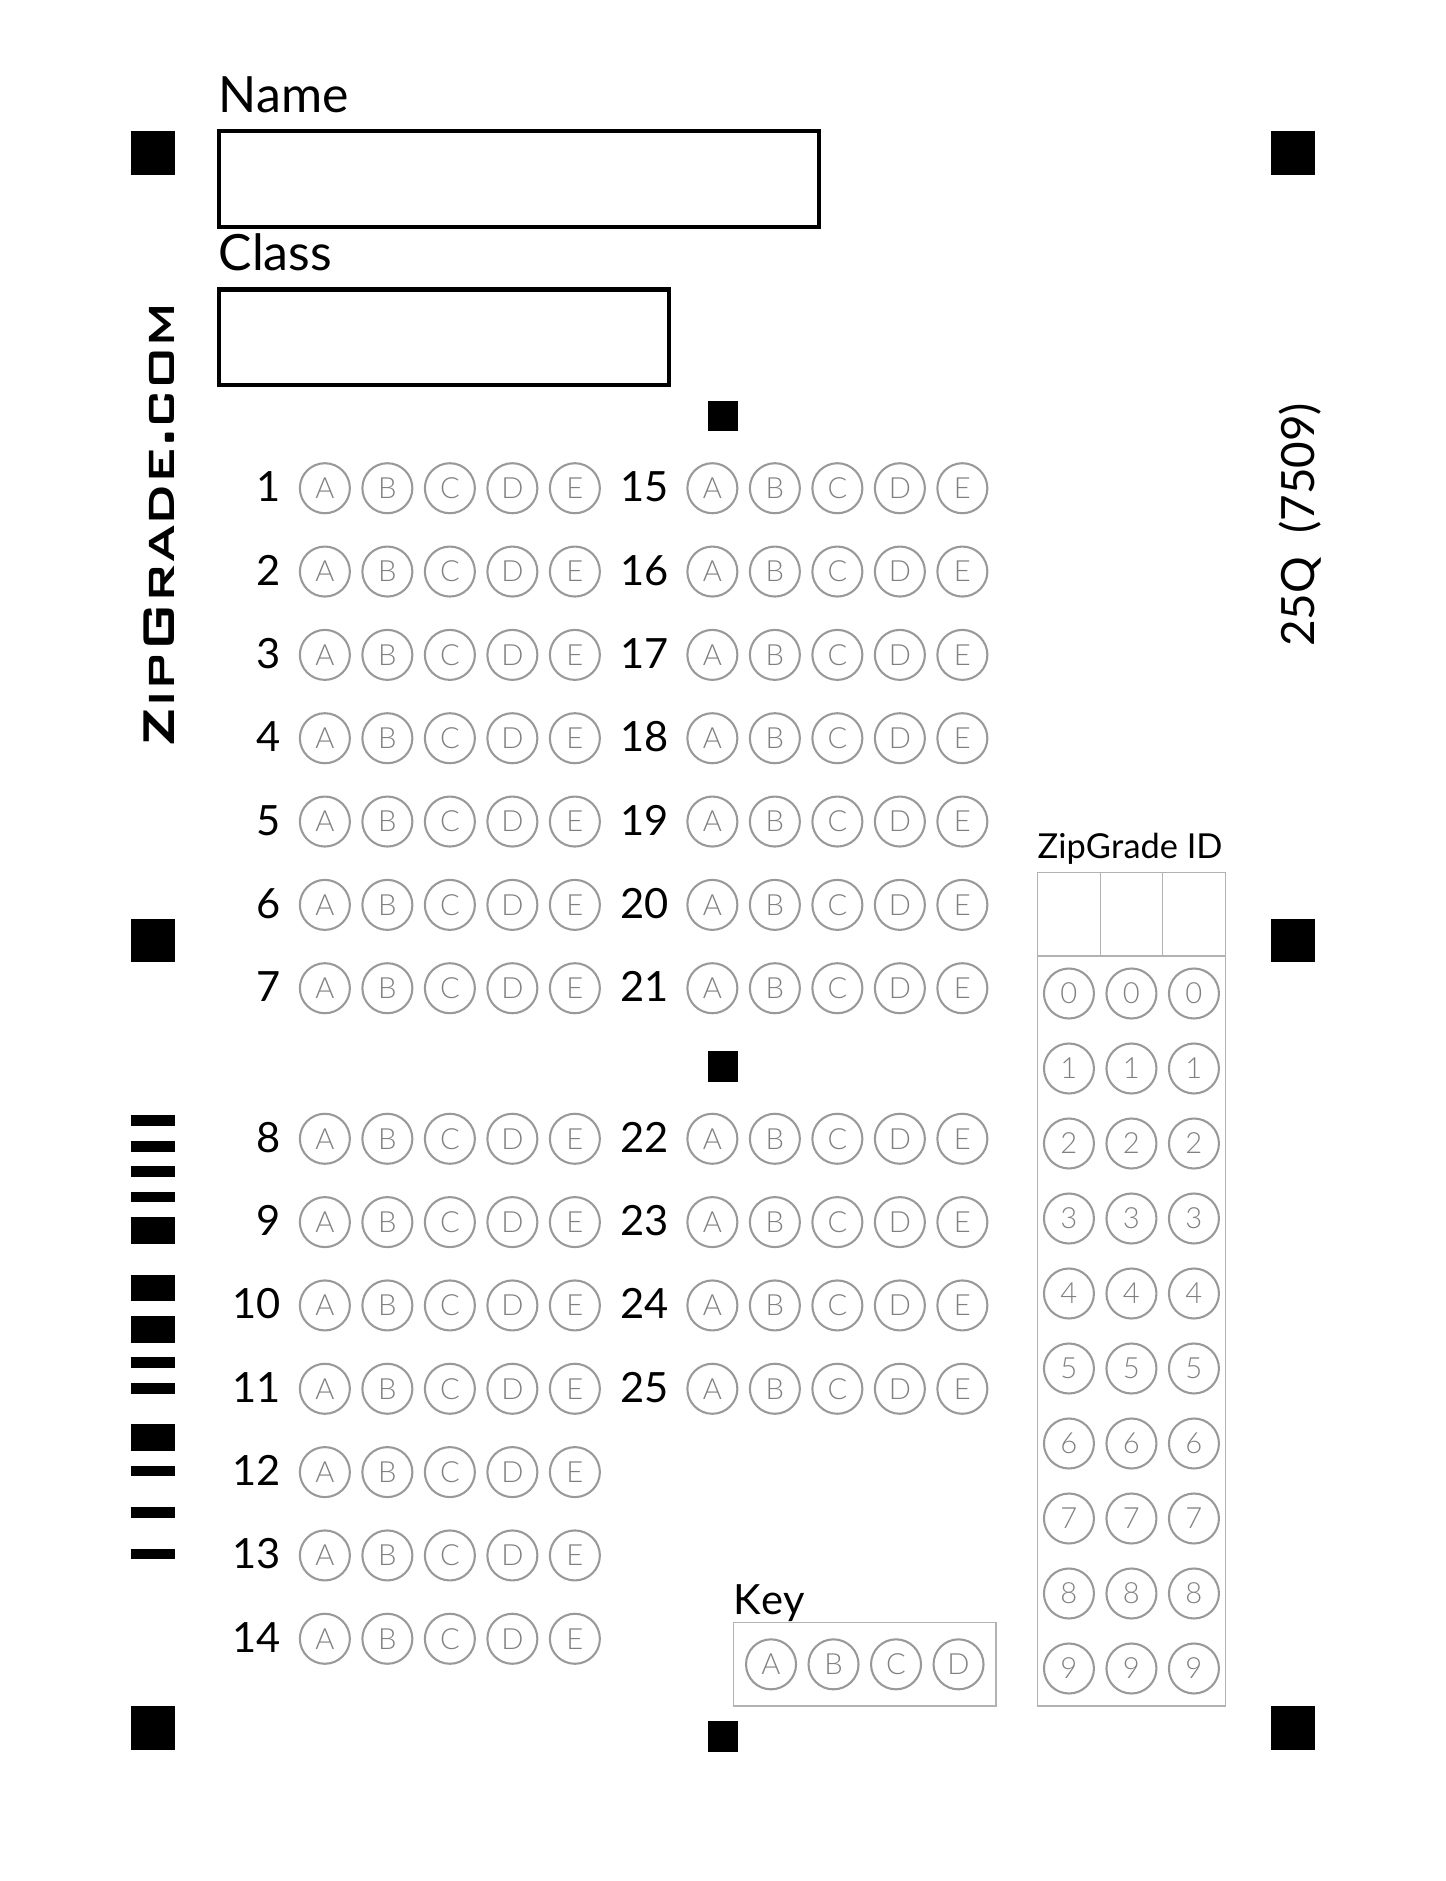
\includegraphics[width=.7\textwidth]{25Q.png}};
      \fill (#1,#2) circle (0.2);
    \end{tikzpicture}
  \end{flushright}
  \bottommatter
}


  \topmatter
  \drawscantron{6.3}{1.85}


\pagebreak

  \topmatter
  \drawscantron{6.8}{1.85}
  

\pagebreak

  \topmatter
  \drawscantron{7.3}{1.85}

\pagebreak

  \topmatter
  \drawscantron{7.8}{1.85}

\end{document}